% Signal Scissors -- CSE 220 Final Project Presentation
% Compile with pdflatex (or upload this whole `presentation/` folder to Overleaf
% as a project and set main.tex as the main document).
\documentclass[aspectratio=169,10pt]{beamer}

\usetheme{metropolis}
\usepackage[utf8]{inputenc}
\usepackage[T1]{fontenc}
\usepackage{tikz}
\usetikzlibrary{arrows.meta, positioning, fit, backgrounds}
\usepackage{amsmath}
\usepackage{graphicx}
\usepackage{booktabs}
\usepackage{array}

% ---- Colors: clean, modern, high-contrast accent (works in light & projector) ----
\definecolor{ssBlue}{HTML}{2563EB}
\definecolor{ssTeal}{HTML}{0EA5A4}
\definecolor{ssInk}{HTML}{111827}
\definecolor{ssGray}{HTML}{6B7280}

\setbeamercolor{palette primary}{bg=ssBlue, fg=white}
\setbeamercolor{frametitle}{bg=ssBlue, fg=white}
\setbeamercolor{progress bar}{fg=ssTeal, bg=ssGray!25}
\setbeamercolor{normal text}{fg=ssInk}
\setbeamercolor{alerted text}{fg=ssBlue}
\setbeamertemplate{frame footer}{Signal Scissors --- CSE 220}
\metroset{block=fill, progressbar=frametitle, numbering=fraction, sectionpage=none}

% Consistent small helper for source-file citations under diagrams/bullets
\newcommand{\srcnote}[1]{{\scriptsize\color{ssGray}\texttt{#1}}}

\title{Signal Scissors}
\subtitle{An Interactive Workstation for Signals \& LTI Systems}
\author{Al Arafat Alif \textbar\ 2305062 \and Safwan Bin Ahmadul Hoque \textbar\ 2305087}
\institute{CSE 220 --- Signals \& Systems Sessional \\ Department of CSE, BUET}
\date{Final Project Evaluation}

\begin{document}

% Slide 1 -- Title (presenter: Alif, ~10s)
\begin{frame}
  \titlepage
\end{frame}

% Slide 2 -- Motivation & Approach (presenter: Alif, ~25s)
\begin{frame}{Motivation \& Approach}
  \begin{columns}[T, totalwidth=\textwidth]
    \begin{column}{0.48\textwidth}
      \alert{The Problem}
      \begin{itemize}
        \item Audio DSP feels like a \alert{black box} or a chalkboard equation
        \item Hard to connect $X[k]$, $h[n]$, filters to what you actually hear
      \end{itemize}
    \end{column}
    \begin{column}{0.48\textwidth}
      \alert{Our Approach}
      \begin{itemize}
        \item Load, synthesize, or record a signal
        \item Apply real FFT / LTI operations
        \item \alert{See it \& hear it}, instantly, side by side
      \end{itemize}
    \end{column}
  \end{columns}
  \vspace{0.6cm}
  \centering
  {\large\alert{Signal Scissors} turns Fourier filtering and LTI systems into something tangible.}
\end{frame}

% Slide 3 -- Theory (presenter: Safwan, ~30s)
\begin{frame}{Theory in Action}
  \small
  \begin{columns}[T, totalwidth=\textwidth]
    \begin{column}{0.55\textwidth}
      \textbf{DFT / FFT band filter}
      \[
        X[k] = \sum_{n=0}^{N-1} x[n]\, e^{-j2\pi kn/N}
      \]
      \vspace{-0.15cm}
      \textbf{LTI convolution echo}
      \[
        y[n] = x[n] * h[n]
      \]
      \vspace{-0.15cm}
      \textbf{Amplitude scale \& time shift}
      \[
        y[n] = A\,x[n], \qquad y[n] = x[n - n_0]
      \]
    \end{column}
    \begin{column}{0.42\textwidth}
      \begin{itemize}
        \item FFT $\rightarrow$ mask band $\rightarrow$ IFFT
        \item Cut / Keep / Attenuate / Amplify
        \item $h[n]$: decaying spaced impulses
        \item Analytic signal (Hilbert-style) $\rightarrow$ SSB freq.\ shift
        \item STFT $\rightarrow$ time--frequency spectrogram
      \end{itemize}
    \end{column}
  \end{columns}
  \vspace{0.25cm}
  \srcnote{fourier\_filter.py $\cdot$ audio\_effects.py $\cdot$ server.py (frequency\_shift\_channel, compute\_spectrogram\_payload)}
\end{frame}

% Slide 4 -- Backend Architecture & Signal Flow (presenter: Safwan, ~30s)
\begin{frame}{Backend Architecture \& Signal Flow}
  \centering
  \resizebox{\linewidth}{!}{%
  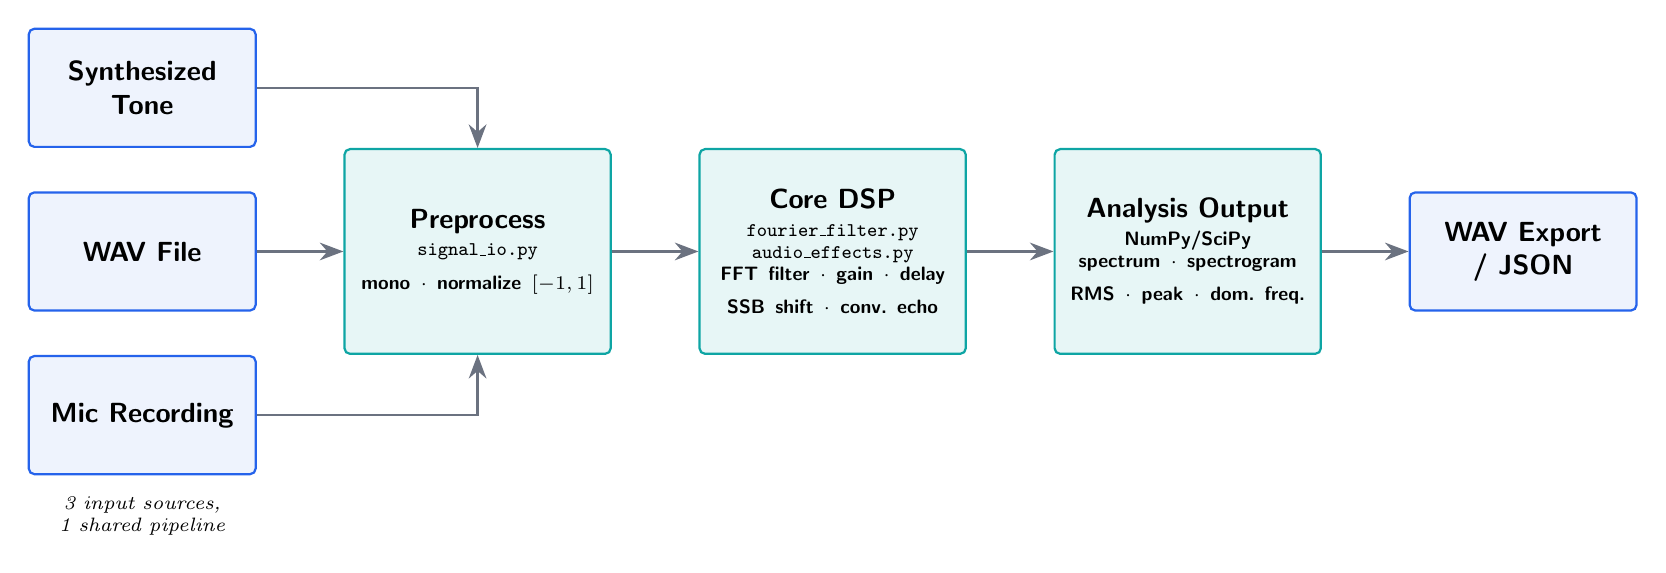
\begin{tikzpicture}[
      node distance=0.55cm and 0.65cm,
      every node/.style={font=\sffamily\bfseries},
      box/.style={draw=ssBlue, thick, rounded corners=2pt, fill=ssBlue!8,
                   align=center, minimum height=1.5cm, text width=2.6cm, inner sep=4pt},
      stage/.style={draw=ssTeal, thick, rounded corners=2pt, fill=ssTeal!10,
                    align=center, minimum height=2.6cm, text width=3.1cm, inner sep=4pt},
      arr/.style={-{Stealth[length=3mm]}, thick, draw=ssGray}
    ]
    % --- Input column (stacked) ---
    \node[box] (file) {WAV File};
    \node[box, below=of file] (mic) {Mic Recording};
    \node[box, above=of file] (synth) {Synthesized Tone};

    \node[stage, right=1.1cm of file] (pre) {Preprocess\\[2pt] \scriptsize \texttt{signal\_io.py}\\ mono $\cdot$ normalize $[-1,1]$};
    \node[stage, right=1.1cm of pre] (dsp) {Core DSP\\[2pt] \scriptsize \texttt{fourier\_filter.py}\\ \texttt{audio\_effects.py}\\ FFT filter $\cdot$ gain $\cdot$ delay\\ SSB shift $\cdot$ conv.\ echo};
    \node[stage, right=1.1cm of dsp] (viz) {Analysis Output\\[2pt] \scriptsize NumPy/SciPy\\ spectrum $\cdot$ spectrogram\\ RMS $\cdot$ peak $\cdot$ dom.\ freq.};
    \node[box, right=1.1cm of viz, minimum height=1.5cm] (out) {WAV Export\\ /\ JSON};

    \draw[arr] (synth) -| (pre);
    \draw[arr] (file) -- (pre);
    \draw[arr] (mic) -| (pre);
    \draw[arr] (pre) -- (dsp);
    \draw[arr] (dsp) -- (viz);
    \draw[arr] (viz) -- (out);

    \node[below=0.15cm of mic, font=\scriptsize\itshape, text width=2.6cm, align=center, draw=none, fill=none] {3 input sources, 1 shared pipeline};
  \end{tikzpicture}%
  }

  \vspace{0.35cm}
  \small
  \textbf{Signal flow:}\ Load/Record/Synthesize $\rightarrow$ Set Filter/Effect Parameters $\rightarrow$ Apply (FFT/LTI math) $\rightarrow$ Compare Original vs.\ Processed

  \vspace{0.15cm}
  \srcnote{All DSP is plain NumPy/SciPy --- \texttt{server.py}, \texttt{fourier\_filter.py}, \texttt{audio\_effects.py}, \texttt{signal\_io.py}}
\end{frame}

% Slide 5 -- Features (presenter: Alif, ~25s)
\begin{frame}{Features}
  \footnotesize
  \begin{columns}[T, totalwidth=\textwidth]
    \begin{column}{0.25\textwidth}
      \textbf{Control Center}
      \begin{itemize}
        \item Browse a WAV file
        \item Record from mic
        \item Synthetic presets
      \end{itemize}
    \end{column}
    \begin{column}{0.25\textwidth}
      \textbf{Spectral Studio}
      \begin{itemize}
        \item Cut / keep / attenuate / amplify
        \item Gain, delay, SSB shift
        \item Convolution echo
      \end{itemize}
    \end{column}
    \begin{column}{0.25\textwidth}
      \textbf{Real-Life Applications}
      \begin{itemize}
        \item 11 one-click scenarios
        \item Telephone filter, hum notch
        \item Reverb, hearing-aid boost
      \end{itemize}
    \end{column}
    \begin{column}{0.25\textwidth}
      \textbf{Signal Inspector}
      \begin{itemize}
        \item Spectrum \& $\Delta$dB
        \item Waveform overlay
        \item STFT spectrogram
      \end{itemize}
    \end{column}
  \end{columns}
  \vspace{0.3cm}
  \srcnote{Real-Life Applications sends the identical filter/effects parameters to the same backend DSP functions as Spectral Studio --- curated values, not a separate engine}
\end{frame}

% Slide 6 -- Implementation Decisions (presenter: Safwan, ~30s)
\begin{frame}{Key Implementation Decisions}
  \begin{itemize}
    \item \alert{3 input sources, 1 pipeline}: synthesizer (known ground-truth frequencies) $\cdot$ file (real-world audio) $\cdot$ mic (live input) --- all normalized identically before processing
    \item \alert{11 Real-Life Application presets} (telephone filter, hum notch, reverb, hearing-aid boost, \ldots) call the \emph{same} filter/effects functions --- just curated parameters, not a separate engine
    \item Spectrum always plotted \alert{0 to $f_s/2$} (Nyquist) --- correct one-sided FFT magnitude
    \item Convolution echo output is \alert{soft-clipped with $\tanh(\cdot)$}, not hard-normalized --- preserves the decaying reflection tail instead of squashing it flat
    \item \alert{Challenge solved}: STFT spectrogram rendered solid black --- root cause was a fixed $-80$ to $0$\,dB color scale vs.\ SciPy's PSD output ($\approx\!-120$ to $-60$\,dB); fixed by scaling color range to the data's own peak
  \end{itemize}
\end{frame}

% Slide 7 -- Results (presenter: Alif, ~25s)
\begin{frame}{Results}
  \begin{columns}[T, totalwidth=\textwidth]
    \begin{column}{0.5\textwidth}
      \centering
      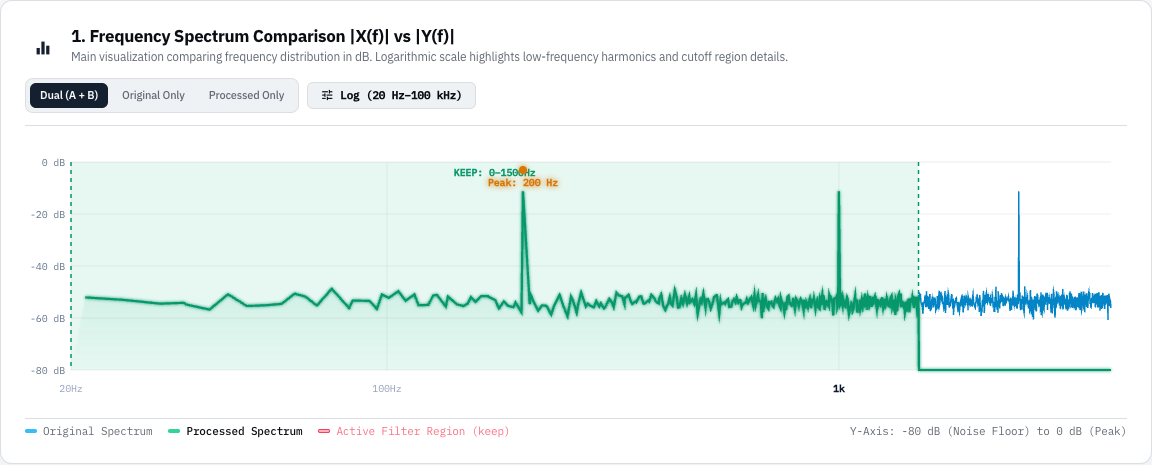
\includegraphics[width=\linewidth]{images/inspector_spectrum_comparison.png}
      \vspace{2pt}

      \footnotesize Multi-tone (200/1000/2500\,Hz) through a 0--1500\,Hz \emph{Keep} filter --- the 2500\,Hz peak is removed
    \end{column}
    \begin{column}{0.5\textwidth}
      \centering
      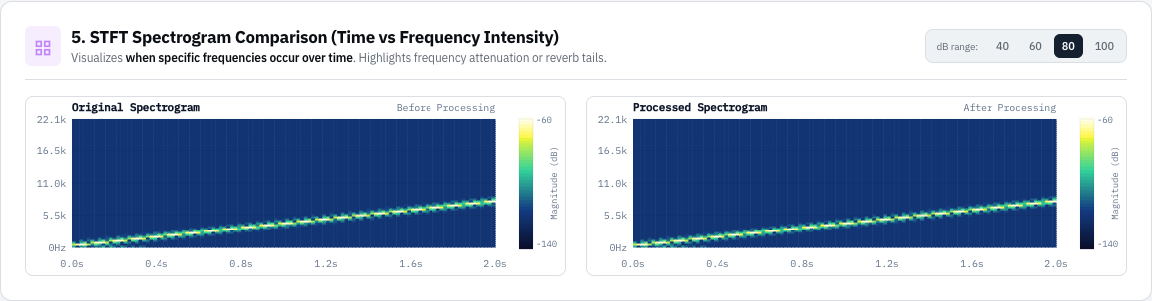
\includegraphics[width=\linewidth]{images/inspector_spectrogram_chirp.png}
      \vspace{2pt}

      \footnotesize Linear chirp, 200\,Hz $\to$ 8000\,Hz over 2\,s --- rising diagonal in the STFT spectrogram
    \end{column}
  \end{columns}
\end{frame}

% Slide 8 -- Live Demo (both presenters, ~10s setup then ~2 min live)
\begin{frame}{Live Demo}
  \begin{enumerate}
    \item Load the \alert{Standard Multi-Tone} preset (Control Center)
    \item Apply \alert{"Vintage Telephone Bandwidth Filter"} --- a Real-Life Application preset (Acoustic FX Engine)
    \item Compare original vs.\ processed \alert{spectrum} (Signal Inspector)
    \item View the \alert{STFT spectrogram}
  \end{enumerate}
  \vspace{0.4cm}
  \centering
  {\Large\alert{Switching to the live app now\ldots}}
\end{frame}

% Slide 9 -- Conclusion & Thank You (presenter: Safwan, ~15s)
\begin{frame}{Conclusion \& Future Work}
  \begin{columns}[T, totalwidth=\textwidth]
    \begin{column}{0.5\textwidth}
      \textbf{Conclusion}
      \begin{itemize}
        \item FFT filtering \& LTI systems made visual, audible, interactive
        \item One pipeline, three ways in: file, mic, synthesizer
      \end{itemize}
    \end{column}
    \begin{column}{0.5\textwidth}
      \textbf{Future Work}
      \begin{itemize}
        \item Real-time streaming DSP
        \item More filter families (IIR, custom windows)
      \end{itemize}
    \end{column}
  \end{columns}

  \vspace{0.7cm}
  \centering
  {\Huge\alert{Thank You}}\\[6pt]
  {\Large Questions?}
\end{frame}


\end{document}
